\section{Data Analysis}
\setlength{\parindent}{10ex}

All data used in this work was aggregated from exsisting studies.
The ETOPO dataset was used for bathymetry soundings \cite{national1988etopo}.
All other features and their origin datasets can be seen in the table below. %Insert point to figure yadaydada

%This section is for defining the data being used in the experiment
%It should define where the data came from and its format
%I can also explain any of the special stuff I am doing (Binning for example)
%

\begin{center}
    \begin{table}[htb]
        \begin{tabular}{ |p{0.5\textwidth} p{0.5\textwidth}| }
            \hline
                \textbf{Feature} & \textbf{Origin Study} \\
                Mantle Density & CRUST1 \cite{laske2013update} \\
                LAND One Hot & ETOPO \cite{national1988etopo} \\
                Crust Thickness & CRUST1 \cite{laske2013update} \\
                Low, Mid, High Crust Density & CRUST1 \cite{laske2013update} \\
                Estimated Current East, North, Mag & HYCOM \cite{chassignet2009us} \\
                Sea Nitrate, Phosphate, Salinity Measurements & NASA Studies \cite{meissner2018salinity} \cite{parekh2005decoupling}  \\
                Sea Temperature, Silicate Measurements & NASA Studies \\
                Sediment Thickness & CRUST1 \cite{laske2013update} \\
                BioMass Features & \cite{wei2010global} \\
                Geoid Features & EGM \cite{pavlis2008earth} \\
                Wave height, period & WAVEWATCH \cite{tolman20072007} \\
            \hline
        \end{tabular}
        \label{table:FEATURE_LIST}
        \caption{List of Ocean Features used in Models for this Project.}
    \end{table}
\end{center}
%I am using this section to introduce the feature selection method that I preformed
%Maybe I can flesh this out more and talk about it in def??
%Maybe make a diagram for the flow of the GA?
\subsection{Feature Selection}
Feature selection was used to identify the most relevant features for classification.
This important step in the \ac{ML} pipline removes noise from irrelevant data.
This work used a genetic algorithm approach for feature selection \cite{yang1998feature}.
Other approaches that where considered included a grid search, dimensional analysis, and simple variable correlations.
These approaches were found to either take to long, or simply not offer enough improvement to the model.
Where as, the genetic algorithm approach gave relativly quick model improvements with little effort.
See \ref{fig:GA} for an illustration of a generic genetic algorithm.

\par
Using a genetic algorithm for feature selection is a simple application of the original process.
The initialized population is a set of random binary strings.
Each string has a character length equal to the number of features in our feature space.
The binary characters represent if a feature is active or inactive.
Essentially these strings represent a set of features to use in training a model.
The fittness of that string is represented by the resulting models accuracy.
Selection is preformed by choosing the most accurate models, and their characteristics are passed to the next generation.
A simple crossover mutation of the strings is used, along with a modest 5 percent mutation rate.
Upon termination the resulting fittest string is used as the selected features.


\begin{center}
    \begin{figure}[h]
        \caption{Diagram of Generic Genetic Algorithm}
        \label{fig:GA}
        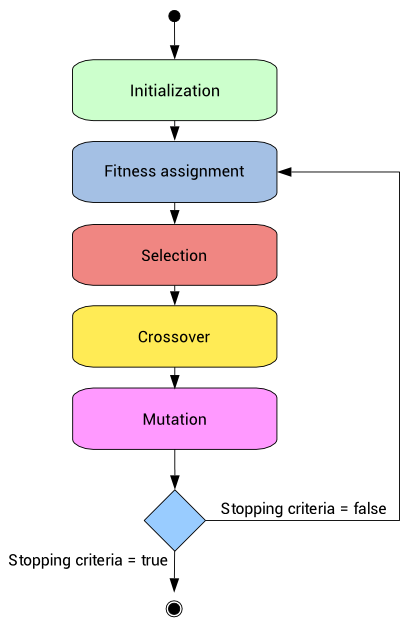
\includegraphics{genetic_algorithm.png}
    \end{figure}
\end{center}

%This decribes how the grid files are used and oragnized...
%They are essentially binary files...
\subsection{Data Representation}
Representing global data is typically done using a grid.
Where each grid represents a coverage of the Earth's surface.
This representation can an average of the data across the coverage of that cell, but is not garunteed.
The data used in this work has been organized into a grid for this purpose.
Each grid represents a cell centered data point, and they are oragnized into a EPSG:3857 \ac{CRS}.

\par
The spatial resolution of a grid defines its coverage.
This spatial resolution can be described as the height and width of a grid.
This height and width is not physicaly constant.
For example, a cell at the equator is larger and covers more physical area than a cell at the poles.
However, this is the best way to represent the data in a consistent and structured manner.

\par
All data in this project has been oragnized into two minute bathymetry grids.
A two minute bathymetry grid has a spatial resolution of 0.034 degrees per cell.
This is approximately 3 kilometers of spatial coverage.
The grids have a column length of 5400 and a row width of 10800.

\par
This resolution was chosen for experiments to conserve memory and time.
Larger grids have a exponentially larger memory and computatiional footprint.
I used the \ac{ETOPO}2v2 \cite{national1988etopo} dataset as the source of the two minute bathymetry grid.
Finer resolution datasets exsist, such as the SRMT30 \cite{becker2009global} at 30 second resolution.
However, portions of data in that set is upsampled from lower resolution datasets such as ETOPO.
In any event, the two minute resolution offered a good balance of memory, accuracy, and computational costs.

\subsection{Ocean Features}
Similar to bathymetry values, all extracted ocean features for this project were organized into a two minute bathymetry grid.
They were aggregated from several projects.
Absent data points was either interpolated, or filled with default values.
See \ref{table:FEATURE_LIST} for a complete list of all features.

\par
\ref{fig:bathyxfish} shows the relationship between estimated fish biomass and bathymetry.
There is a direct relationship that trends toward less biomass as the ocean gets deeper.
Naturaly, this relationship is explained by the availability of food and light at such lower depths.
\ref{fig:bathyxfauna} shows a similar relationship to the fish biomass.

\par
\ref{fig:bathyxdensity} shows a example of a inverse relationship to bathymetry.
\ref{fig:pairplot} Shows a pairplot of all the features used in training.
The diagnol in the pair plot will show the correlation of point distributions in each individual plot.
Each of the discussed plots were taken from data in the south Pacific ocean.
This was done as a isolated demonstration of the data.
%Talk about the plots here and include them once seaborn has decided to stop being dumb...

\begin{figure}[h]
    \centering
    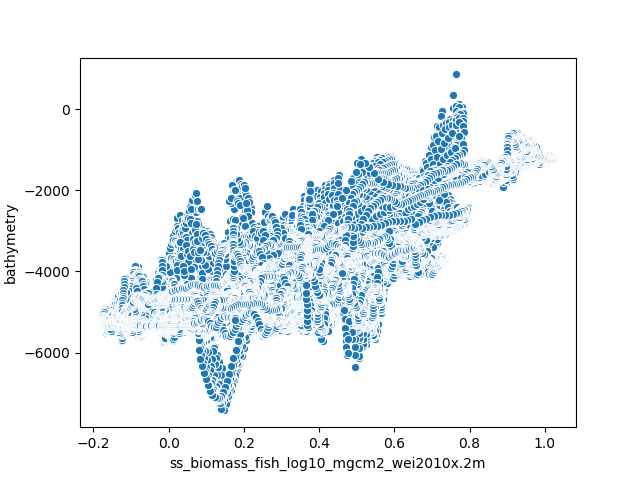
\includegraphics{Bathymetry_X_SS_BIOMASS_FISH_LOG10_MGCM2_Wei2010x.png}
    \caption{Graph of Bathymetry and Estimated Fish BIOMASS}
    \label{fig:bathyxfish}
\end{figure}

\begin{figure}[h]
    \centering
    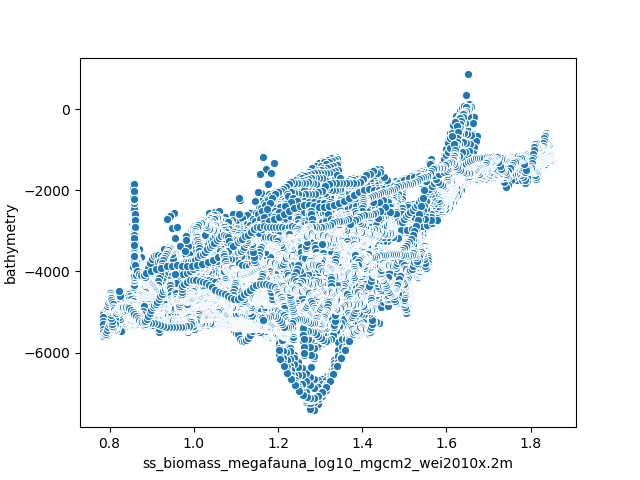
\includegraphics{Bathymetry_X_SS_BIOMASS_MEGAFAUNA_LOG10_MGCM2_Wei2010x.png}
    \caption{Graph of Bathymetry and Estimated MegaFauna Bio Mass}
    \label{fig:bathyxfauna}
\end{figure}

\begin{figure}[h]
    \centering
    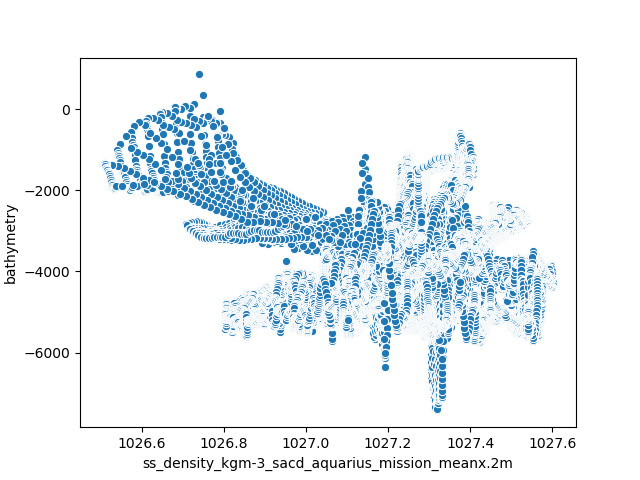
\includegraphics{Bathymetry_X_SS_DENSITY_KGM-3_SACD_Aquarius_MISSION_MEANx.png}
    \caption{Graph of Bathymetry and Estimated Crust Density}
    \label{fig:bathyxdensity}
\end{figure}

\begin{figure}[h]
    \centering
    \includegraphics{pairplot.png}
    \caption{Pair Plot of All Features Used in Training}
    \label{fig:pairplot}
\end{figure}

%Maybe I can talk about some of the correlations I preformed here???? A few graphs perhaps???
%Maybe talk about the PCC???
%Possibly need to talk about the breadth of features here....

\subsection{Bathymetry Values}
ETOPO2v2 is used for the bathymetry soundings \cite{national20062}.
This extention of the ETOPO2 dataset \cite{national1988etopo} is a more accurate and updated version of the ETOPO2 dataset.
Specifically this version elimates a westward bias present in the original version.
The two minue \ac{ETOPO} dataset was used to match the chosen resolution for this work.
\ac{ETOPO} was aggregated by the \ac{NGDC} which is a department of \ac{NOAA}.

\par
Land topography is included in the \ac{ETOPO} dataset.
A mask was created to mask out the land topography in all training datasets.
The masking is the LAND One hots feature listed in \ref{table:FEATURE_LIST}.
This is applied to the data before training.

%There is a better was to describe why the features were binned like this
%I want to describe the value that was added by binning my data into classes!
\par
The classification preformed in this work used binned bathymetry from \ac{ETOPO}.
These classes where partioned on a interval of 150 meters.
This partitioning scheme was chosen to improve upon the results from a similar project \cite{jena2012prediction}.
The binning is preformed to leverage the unique advantages inherient to classification problems and test if this problem is better suited for classification.
For example, the use of metrics such as a confusion matrix makes comparing the preformance of the model signifigantly easier.